\documentclass{article}\usepackage[]{graphicx}\usepackage[]{color}
% maxwidth is the original width if it is less than linewidth
% otherwise use linewidth (to make sure the graphics do not exceed the margin)
\makeatletter
\def\maxwidth{ %
  \ifdim\Gin@nat@width>\linewidth
    \linewidth
  \else
    \Gin@nat@width
  \fi
}
\makeatother

\definecolor{fgcolor}{rgb}{0.345, 0.345, 0.345}
\newcommand{\hlnum}[1]{\textcolor[rgb]{0.686,0.059,0.569}{#1}}%
\newcommand{\hlstr}[1]{\textcolor[rgb]{0.192,0.494,0.8}{#1}}%
\newcommand{\hlcom}[1]{\textcolor[rgb]{0.678,0.584,0.686}{\textit{#1}}}%
\newcommand{\hlopt}[1]{\textcolor[rgb]{0,0,0}{#1}}%
\newcommand{\hlstd}[1]{\textcolor[rgb]{0.345,0.345,0.345}{#1}}%
\newcommand{\hlkwa}[1]{\textcolor[rgb]{0.161,0.373,0.58}{\textbf{#1}}}%
\newcommand{\hlkwb}[1]{\textcolor[rgb]{0.69,0.353,0.396}{#1}}%
\newcommand{\hlkwc}[1]{\textcolor[rgb]{0.333,0.667,0.333}{#1}}%
\newcommand{\hlkwd}[1]{\textcolor[rgb]{0.737,0.353,0.396}{\textbf{#1}}}%
\let\hlipl\hlkwb

\usepackage{framed}
\makeatletter
\newenvironment{kframe}{%
 \def\at@end@of@kframe{}%
 \ifinner\ifhmode%
  \def\at@end@of@kframe{\end{minipage}}%
  \begin{minipage}{\columnwidth}%
 \fi\fi%
 \def\FrameCommand##1{\hskip\@totalleftmargin \hskip-\fboxsep
 \colorbox{shadecolor}{##1}\hskip-\fboxsep
     % There is no \\@totalrightmargin, so:
     \hskip-\linewidth \hskip-\@totalleftmargin \hskip\columnwidth}%
 \MakeFramed {\advance\hsize-\width
   \@totalleftmargin\z@ \linewidth\hsize
   \@setminipage}}%
 {\par\unskip\endMakeFramed%
 \at@end@of@kframe}
\makeatother

\definecolor{shadecolor}{rgb}{.97, .97, .97}
\definecolor{messagecolor}{rgb}{0, 0, 0}
\definecolor{warningcolor}{rgb}{1, 0, 1}
\definecolor{errorcolor}{rgb}{1, 0, 0}
\newenvironment{knitrout}{}{} % an empty environment to be redefined in TeX

\usepackage{alltt}

\usepackage{float}

% Set the margins on the page to not be so large
\addtolength{\oddsidemargin}{-.875in}
\addtolength{\evensidemargin}{-.875in}
\addtolength{\textwidth}{1.75in}
\addtolength{\topmargin}{-.875in}
\addtolength{\textheight}{1.75in}

% Take off page numbering
\pagenumbering{gobble}
\IfFileExists{upquote.sty}{\usepackage{upquote}}{}
\begin{document}

\title{%
  7.1.1 - R: Principal Component Regression, Quantile Regression \\
  \smallskip
  \large Stat 5100: Dr. Bean
}
\date{}

\maketitle

\subsection{Principal Components}

\textbf{Example:} Baseball, same as Handout 4.1.1 Ex. 2

\begin{knitrout}
\definecolor{shadecolor}{rgb}{0.969, 0.969, 0.969}\color{fgcolor}\begin{kframe}
\begin{alltt}
\hlkwd{library}\hlstd{(stat5100)}
\hlkwd{data}\hlstd{(baseball)}

\hlcom{# Look at multicollinearity in the baseball dataset}
\hlstd{baseball_lm} \hlkwb{<-} \hlkwd{lm}\hlstd{(logSalary} \hlopt{~} \hlstd{nAtBat} \hlopt{+} \hlstd{nHits} \hlopt{+} \hlstd{nHome} \hlopt{+} \hlstd{nRuns} \hlopt{+} \hlstd{nRBI} \hlopt{+} \hlstd{nBB} \hlopt{+}
                    \hlstd{YrMajor} \hlopt{+} \hlstd{CrAtBat} \hlopt{+} \hlstd{CrHits} \hlopt{+} \hlstd{CrHome} \hlopt{+} \hlstd{CrRuns} \hlopt{+} \hlstd{CrRbi} \hlopt{+}
                    \hlstd{CrBB} \hlopt{+} \hlstd{nOuts} \hlopt{+} \hlstd{nAssts} \hlopt{+} \hlstd{nError,} \hlkwc{data} \hlstd{= baseball)}
\hlstd{olsrr}\hlopt{::}\hlkwd{ols_vif_tol}\hlstd{(baseball_lm)}
\end{alltt}
\begin{verbatim}
##    Variables   Tolerance        VIF
## 1     nAtBat 0.046562403  21.476555
## 2      nHits 0.035153418  28.446736
## 3      nHome 0.129349044   7.731020
## 4      nRuns 0.068765678  14.542138
## 5       nRBI 0.087218325  11.465480
## 6        nBB 0.251956556   3.968938
## 7    YrMajor 0.108262158   9.236838
## 8    CrAtBat 0.004002379 249.851404
## 9     CrHits 0.002011778 497.072822
## 10    CrHome 0.019972282  50.069392
## 11    CrRuns 0.006210431 161.019424
## 12     CrRbi 0.007421451 134.744542
## 13      CrBB 0.048834939  20.477142
## 14     nOuts 0.795937680   1.256380
## 15    nAssts 0.368119153   2.716512
## 16    nError 0.455458468   2.195590
\end{verbatim}
\end{kframe}
\end{knitrout}

\subsubsection*{Consider using principal components}

\begin{knitrout}
\definecolor{shadecolor}{rgb}{0.969, 0.969, 0.969}\color{fgcolor}\begin{kframe}
\begin{alltt}
\hlcom{# Extract the principal components of the baseball dataset}
\hlstd{X} \hlkwb{<-} \hlkwd{subset}\hlstd{(baseball,} \hlkwc{select} \hlstd{=} \hlkwd{c}\hlstd{(}\hlstr{"nAtBat"}\hlstd{,} \hlstr{"nHits"}\hlstd{,} \hlstr{"nHome"}\hlstd{,} \hlstr{"nRuns"}\hlstd{,} \hlstr{"nRBI"}\hlstd{,}
                                 \hlstr{"nBB"}\hlstd{,} \hlstr{"YrMajor"}\hlstd{,} \hlstr{"CrAtBat"}\hlstd{,} \hlstr{"CrHits"}\hlstd{,} \hlstr{"CrHome"}\hlstd{,}
                                 \hlstr{"CrRuns"}\hlstd{,} \hlstr{"CrRbi"}\hlstd{,} \hlstr{"CrBB"}\hlstd{,} \hlstr{"nOuts"}\hlstd{,} \hlstr{"nAssts"}\hlstd{,}
                                 \hlstr{"nError"}\hlstd{))}
\hlstd{X_pc} \hlkwb{<-} \hlkwd{prcomp}\hlstd{(X)}

\hlcom{# To see all 16 principal components, you can directly output the X_pc object.}
\hlcom{# However, this will get really messy so don't worry too much about this}
\hlcom{# output. We mostly care about the first few principal components anyway.}
\hlstd{X_pc}
\end{alltt}
\begin{verbatim}
## Standard deviations (1, .., p=16):
##  [1] 2475.093969  286.973514  165.686115  137.562491  116.131778   93.554968
##  [7]   65.435375   38.257691   13.319198   12.495383   11.352026   10.144714
## [13]    6.376076    4.218704    2.771620    1.592341
## 
## Rotation (n x k) = (16 x 16):
##                   PC1          PC2          PC3          PC4          PC5
## nAtBat   0.0109530283 -0.221777122 -0.594961880 -0.405776341  0.376833418
## nHits    0.0032725701 -0.065381083 -0.176564840 -0.116270232  0.126691737
## nHome    0.0007313881 -0.009911293 -0.004431376 -0.035321575  0.025375304
## nRuns    0.0014815592 -0.033102085 -0.081709273 -0.090732698  0.057130034
## nRBI     0.0027607147 -0.037596699 -0.054369875 -0.094790309  0.082360705
## nBB      0.0021575350 -0.025658587 -0.032879132 -0.088330307 -0.018893170
## YrMajor  0.0018453950  0.001557815  0.004075262  0.003234563 -0.001953785
## CrAtBat  0.9406826033  0.025478229 -0.031817180  0.161248636 -0.026689403
## CrHits   0.2633660844 -0.031076834 -0.065565514  0.080397180  0.198799538
## CrHome   0.0289926501 -0.017485221  0.104723833 -0.298210967  0.092866889
## CrRuns   0.1335533664  0.002527330  0.012604377 -0.279364614 -0.039439398
## CrRbi    0.1300373735 -0.057542279  0.209322493 -0.510317828  0.274722993
## CrBB     0.0998286444  0.017101903  0.210379571 -0.561569915 -0.648355893
## nOuts    0.0072196227 -0.968316437  0.151638201  0.136592107 -0.131239580
## nAssts  -0.0008526885 -0.009613599 -0.689927071  0.040807037 -0.516999469
## nError  -0.0002296318 -0.003489518 -0.024276505  0.001406721 -0.011415177
##                   PC6          PC7          PC8           PC9          PC10
## nAtBat  -0.2963127949 -0.260866564  0.070751902 -0.2741644584 -0.0322488923
## nHits   -0.1111910731 -0.013045989  0.101581142  0.2093141974  0.1291248253
## nHome   -0.0002868509 -0.021463858 -0.020752067  0.2463531166  0.2171610355
## nRuns   -0.0865006860 -0.023749656 -0.030903967  0.3931033427 -0.1638650906
## nRBI    -0.0050311903 -0.039091243  0.040330822  0.7058844460  0.3931730979
## nBB     -0.0659975617 -0.025726296  0.071404087  0.3564240658 -0.4745377143
## YrMajor  0.0030170901 -0.007176650  0.003196113  0.0056223169  0.0037674315
## CrAtBat  0.0245024584 -0.282400459 -0.072927515  0.0205948767 -0.0135990418
## CrHits  -0.1646187791  0.753127221  0.453878040 -0.0739380145  0.1904443996
## CrHome   0.2576889109 -0.040399202 -0.317508430 -0.1631220305  0.6008484644
## CrRuns  -0.2799541438  0.469317254 -0.726363532  0.0519371889 -0.1838421417
## CrRbi    0.6451379949  0.120024535  0.169749419  0.0219779651 -0.2986470224
## CrBB    -0.2967191188 -0.066981727  0.322019204 -0.0611464329  0.0857348473
## nOuts    0.0326403814  0.023872227 -0.041798013 -0.0008592252  0.0006403294
## nAssts   0.4581505278  0.200414262 -0.050549251  0.0321722993  0.0096248996
## nError   0.0165090639  0.006527826  0.001260187  0.0019453713  0.0242159889
##                 PC11         PC12          PC13         PC14          PC15
## nAtBat   0.010072032  0.220723641 -0.0579146541 -0.026605824  0.0056888236
## nHits   -0.217565115 -0.738844269  0.4695533402  0.110369568 -0.1590568258
## nHome    0.007108914  0.134859390 -0.2520185859 -0.084761793 -0.8946023531
## nRuns   -0.006883737 -0.400290616 -0.7553590444 -0.066160127  0.2344128219
## nRBI    -0.151541431  0.416126623  0.1834570731 -0.001756971  0.3066121125
## nBB      0.743253921  0.027208279  0.2582196203  0.036981470 -0.0808982381
## YrMajor -0.008339761 -0.012957986  0.0266979706 -0.035630565 -0.0049305823
## CrAtBat -0.008040060 -0.014457178  0.0123006209  0.003775143 -0.0017106734
## CrHits   0.168479488  0.013173462 -0.0860884601 -0.020311841  0.0301654093
## CrHome   0.525650989 -0.202002100 -0.0596064083 -0.007819106  0.1145473772
## CrRuns  -0.155674066  0.068025547  0.0966892009  0.015691378 -0.0344281365
## CrRbi   -0.215574302  0.045882194  0.0169785210  0.003426238 -0.0457217510
## CrBB    -0.037524682  0.002932373 -0.0304007913 -0.002245537  0.0097592386
## nOuts   -0.004747603 -0.005089937 -0.0005429899 -0.001735777  0.0006844077
## nAssts   0.007389163 -0.007651949 -0.0047646769 -0.032601883 -0.0020035853
## nError   0.007377414  0.069913614 -0.1390630052  0.985439929 -0.0376366642
##                  PC16
## nAtBat   0.0088383253
## nHits   -0.0211086728
## nHome   -0.0009911171
## nRuns    0.0131198188
## nRBI    -0.0044273830
## nBB      0.0005655713
## YrMajor  0.9988005625
## CrAtBat -0.0046140084
## CrHits   0.0074151991
## CrHome   0.0029411893
## CrRuns   0.0048566734
## CrRbi   -0.0012033968
## CrBB    -0.0006083639
## nOuts    0.0002385543
## nAssts   0.0006054241
## nError   0.0396226823
\end{verbatim}
\begin{alltt}
\hlcom{# If we want a more concise summary, we can use the summary function:}
\hlkwd{summary}\hlstd{(X_pc)}
\end{alltt}
\begin{verbatim}
## Importance of components:
##                             PC1       PC2       PC3       PC4       PC5
## Standard deviation     2475.094 286.97351 165.68612 137.56249 116.13178
## Proportion of Variance    0.975   0.01311   0.00437   0.00301   0.00215
## Cumulative Proportion     0.975   0.98806   0.99243   0.99545   0.99759
##                             PC6      PC7      PC8      PC9     PC10     PC11
## Standard deviation     93.55497 65.43538 38.25769 13.31920 12.49538 11.35203
## Proportion of Variance  0.00139  0.00068  0.00023  0.00003  0.00002  0.00002
## Cumulative Proportion   0.99898  0.99967  0.99990  0.99993  0.99995  0.99997
##                            PC12    PC13  PC14  PC15  PC16
## Standard deviation     10.14471 6.37608 4.219 2.772 1.592
## Proportion of Variance  0.00002 0.00001 0.000 0.000 0.000
## Cumulative Proportion   0.99999 1.00000 1.000 1.000 1.000
\end{verbatim}
\end{kframe}
\end{knitrout}

Note that the first principal component represents 97.5\% percent of the total variation in the dataset (this comes from the summary output). This tells us that most likely we can discard all the principal components past the first 2 or so.

\begin{knitrout}
\definecolor{shadecolor}{rgb}{0.969, 0.969, 0.969}\color{fgcolor}\begin{kframe}
\begin{alltt}
\hlcom{# Also show a scree plot}
\hlkwd{screeplot}\hlstd{(X_pc,} \hlkwc{type} \hlstd{=} \hlstr{"lines"}\hlstd{)}
\end{alltt}
\end{kframe}

{\centering 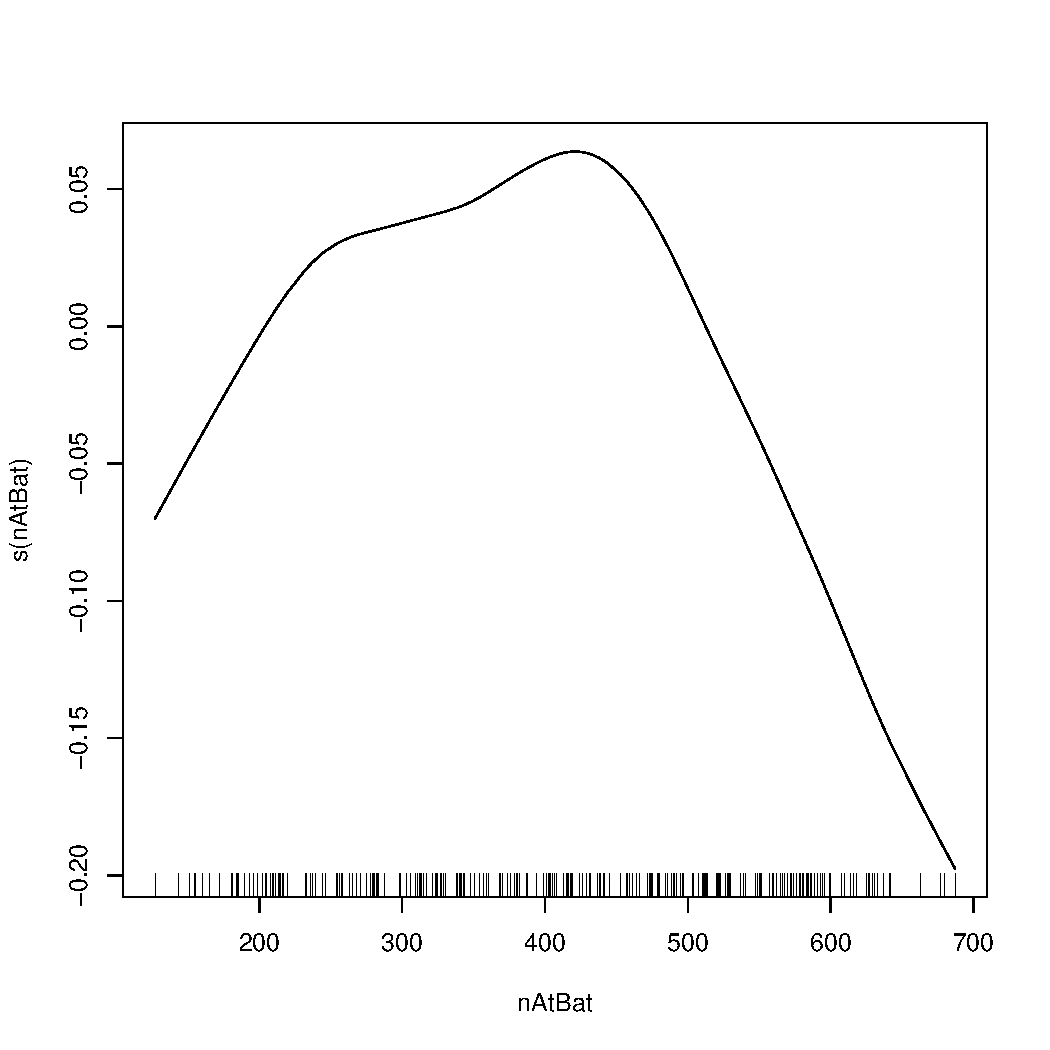
\includegraphics[width=0.6\textwidth]{figure/unnamed-chunk-3-1} 

}



\end{knitrout}

\end{document}
